\subsection{Le parseur}

\begin{frame}{Problématiques et solutions (Parseur)}
    \begin{block}{Problématiques}
        % \begin{itemize}
        %     \item Les classes ne respectaient pas le méta-modèle de CHIPS
        %     \item Ecrit avec Yacc/Bison et Flex $\rightarrow$ supporte pas les templates C++
        % \end{itemize}
        
        \begin{itemize}
            \item Conformité : classes non conformes au méta-modèle de CHIPS.
            \item Limitation : absence de support des templates C++ (Yacc/Bison et Flex).
        \end{itemize}
    \end{block}

{
\setbeamercolor{block title}{fg=white,bg=ufcgreen}

    \begin{block}{Solutions}
        % \begin{itemize}
        %     \item Réécriture des classes avec template C++, passage de 297 classes à 97 classes C++
        %     \item Migration vers ANTLR4 $\rightarrow$ supporte les templates C++
        % \end{itemize}
        
        \begin{itemize}
            \item Réécrire les classes (297 $\rightarrow$ 97 classes C++).
            \item Migrer vers ANTLR4 (support des templates C++).
        \end{itemize}
        
    \end{block}
}

    
\end{frame}

\begin{frame}{Table des symboles (Parseur)}
    \begin{block}{Besoin}
        Une table des symboles assez robuste car il faut pouvoir :
        \begin{itemize}
            \item Interdire d'instancier deux variables ayant le même nom mais un type différent
            \item Interdire des opérations avec deux variables de type différents : \textbf{langage fortement typé}
            \item Vérifier si une variable est accessible dans un scope
        \end{itemize}
    \end{block}
\end{frame}

\begin{frame}{Exemple programme CHIPS}
    \begin{figure}
        \centering
        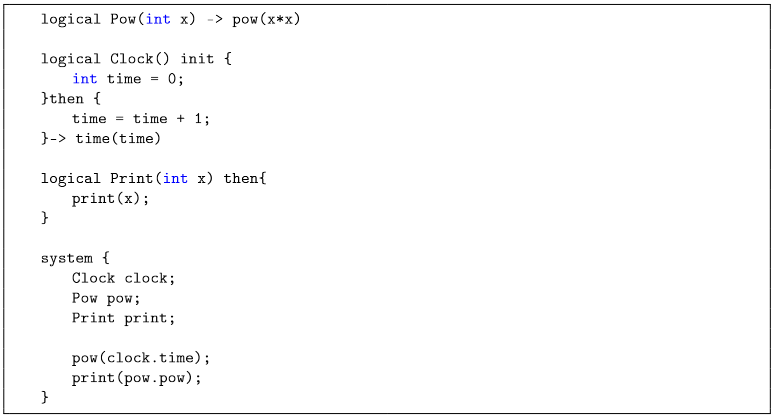
\includegraphics[width=0.8\textwidth]{img/exemple_programme_CHIPS.png}
    \end{figure}
\end{frame}

\begin{frame}{Structure et méthode}
     \begin{block}{Structure interne}
        Repose sur plusieurs niveaux de stockage
        \begin{itemize}
            \item scopes : une pile, chaque scope étant une table associant un nom à un symbole
            \item Symbol qui stocke : valeur réelle , le nom et la catégorie du symbole
            \item Deux tables séparées pour les sorties de fonctions et les paramètres de fonctions
            \item declarated\_block\_system : garde type associé à blocs déclarés
        \end{itemize}
    \end{block}
\end{frame}

\begin{frame}{Structure et méthode}
    \begin{block}{Méthodes}
        \begin{itemize}
            \item enterScope() et exitScope() $\rightarrow$ ouvrir et fermer un scope
            \item declare...() $\rightarrow$ enregistrer un symbole d'un certain genre
            \item lookup...() $\rightarrow$ rechercher un symbole dans les scopes
            \item declareFunctionOutput() et declareFunctionParameter() $\rightarrow$ gérer les données des fonctions
            \item declareBlock() et getTypeOfDeclaratedBlock() $\rightarrow$ mémoriser et lire le type d'un bloc
        \end{itemize}
    \end{block}
\end{frame}

\begin{frame}[fragile]{Exemple d'utilisation de la table des symboles}
  \begin{figure}
        \centering
        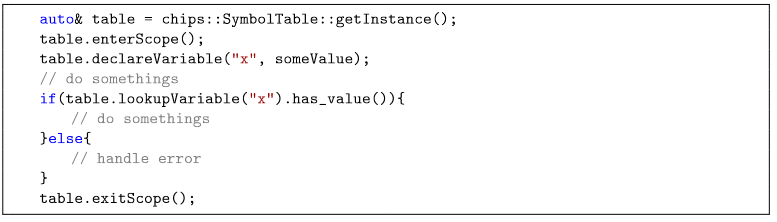
\includegraphics[width=\textwidth]{img/exemple_symboltable_parseur.png}
    \end{figure}
\end{frame}

\subsection{Sérialisation vers XMI}

\begin{frame}{Problématiques et solutions (XMI)}
    \begin{block}{Problématiques}
        % \begin{itemize}
        %     \item Implémentation n'avais pas les nouvelles classes
        %     \item Table des symboles pas assez robuste
        % \end{itemize}
        
        \begin{itemize}
            \item Implémentation : incompatible avec les nouvelles classes.
            \item Table des symboles : robustesse insuffisante.
        \end{itemize}
    \end{block}
    
    
    {
    \setbeamercolor{block title}{fg=white,bg=ufcgreen}
    
    \begin{block}{Solutions}
        % \begin{itemize}
        %     \item Utiliser les nouvelles classes avec le patron visiteur
        %     \item Améliorer la table des symboles $\rightarrow$ l'ancienne avait des conflits si un paramètre et une sortie de fonction avait le même nom
        % \end{itemize}
        \begin{itemize}
            \item Adapter le patron visiteur aux nouvelles classes.
            \item Éliminer les conflits de noms dans la table des symboles.
        \end{itemize}
    \end{block}
    
    }
    
    
\end{frame}
